\documentclass{standalone}
\RequirePackage{tikz}
\RequirePackage{ifthen}
\usetikzlibrary{arrows,shapes}
\tikzstyle{btreeptr} = [draw, ultra thin, fill=blue!50, minimum height=1cm, inner sep=0cm, minimum width=0cm]
\tikzstyle{btreeval} = [draw, semithick, fill=yellow!30, minimum size=1cm]
\tikzstyle{btlink} = [draw, thick, ->, >=triangle 45]
\newcommand{\xyshift}[3]{
  \begin{scope}[xshift=#1, yshift=#2]
    #3
  \end{scope}
}
\newcommand{\btreelink}[2]{
\draw[btlink] (#1.south) -- ([yshift=-0.1cm] #2.north); \&
\fill (#1.south) circle[radius=0.15cm]; \\
}
\newcommand{\btreenodea}[2]{
\matrix [ampersand replacement=\&] (#1)
{
 \node[btreeptr] (#1-a) {\vphantom{1}}; \& \node[btreeval] {#2}; \&
 \node[btreeptr] (#1-b) {\vphantom{1}}; \\
};
}

\begin{document}
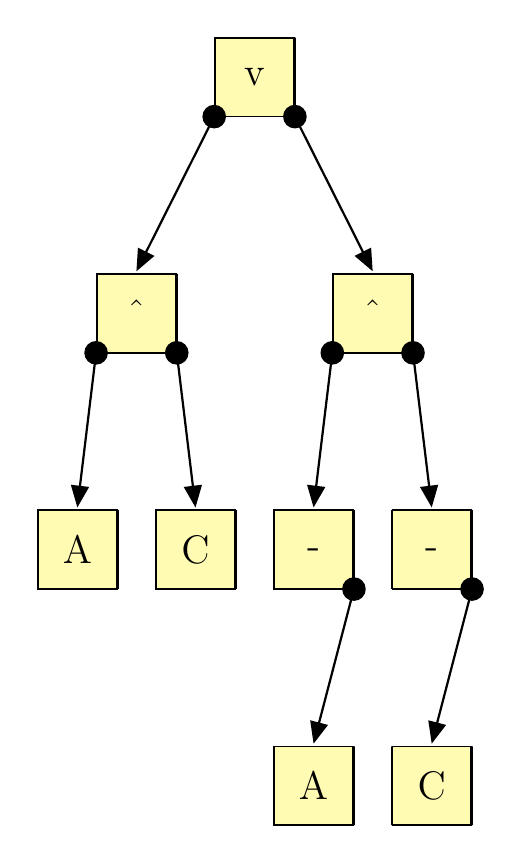
\begin{tikzpicture}
\tikzstyle{every node}=[font=\fontsize{15}{0}\selectfont]
\xyshift{37.5mm}{-90mm}{\btreenodea{j}{A}}
\xyshift{52.5mm}{-90mm}{\btreenodea{bc}{C}}
\xyshift{7.5mm}{-60mm}{\btreenodea{c}{A}}
\xyshift{22.5mm}{-60mm}{\btreenodea{f}{C}}
\xyshift{37.5mm}{-60mm}{\btreenodea{i}{-}}
\xyshift{52.5mm}{-60mm}{\btreenodea{bb}{-}}
\xyshift{15mm}{-30mm}{\btreenodea{b}{\textasciicircum{}}}
\xyshift{45mm}{-30mm}{\btreenodea{h}{\textasciicircum{}}}
\xyshift{30mm}{0mm}{\btreenodea{a}{v}}


\btreelink{i-b}{j}
\btreelink{bb-b}{bc}
\btreelink{b-a}{c}
\btreelink{b-b}{f}
\btreelink{h-a}{i}
\btreelink{h-b}{bb}
\btreelink{a-a}{b}
\btreelink{a-b}{h}
\end{tikzpicture}
\end{document}
